\documentclass[notes]{beamer}
\usepackage[latin1]{inputenc}
\usepackage{tikz}
\usetikzlibrary{arrows}
\usetikzlibrary{shapes.misc}
\usepackage{verbatim}

\title{Ramsey's Theorem \\$\nRightarrow_{\text{soc}}$ Weak Weak Konig's
Lemma}
\author{Li Ling Ko}
\institute{University of Notre Dame}
\date{22 January, 2018}
\setbeamertemplate{footline}[frame number]

\begin{document}
\begin{frame}
  \titlepage
\end{frame}

\begin{frame}{Weak Weak Konig's Lemma (WWKL)}
  \begin{itemize}
    \item Konig's Lemma
    \item Weak Konig's Lemma
    \item Weak Weak Konig's Lemma
    \item Define Lebesgue measure
  \end{itemize}

  \begin{itemize}
    \item Asserts existence of randomness
  \end{itemize}
\end{frame}

\begin{frame}{Ramsey's Theorem ($\text{RT}$)}
  \begin{itemize}
    \item State $\text{RT}_k^n$
    \item $\text{RT}$ is $(\forall n)\; \text{RT}_{<\infty}^n$
  \end{itemize}

  \begin{itemize}
    \item Asserts existence of homogenuity
  \end{itemize}
\end{frame}

\begin{frame}{Strongly Omnisciently Computably Reducible
  ($\leq_{\text{soc}}$)}
  \begin{itemize}
    \item Define problem, solution
    \item Use WWKL/RT to illustrate
    \item Define $\leq_{\text{soc}}$
  \end{itemize}
\end{frame}

\note{
  \begin{itemize}
    \item Mention other reductions
    \item soc doesn't require the second problem to be computable from the
      first one
  \end{itemize}
}

\begin{frame}{RT, KL, WKL, WWKL under $\leq_{\text{soc}}$}
  \begin{itemize}
    \item KL ``stronger than'' RT
    \item Homogeneous ``independent from'' randomness
  \end{itemize}

  \begin{center}
    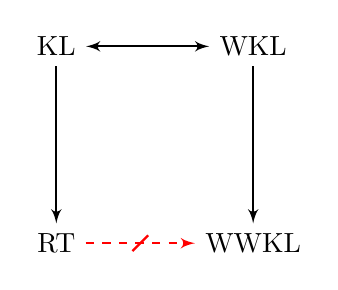
\begin{tikzpicture}[node distance=2.5cm,auto,thick,>=latex']
      \node (KL) {KL};
      \node (WKL) [right of=KL] {WKL};
      \node (WWKL) [below of=WKL] {WWKL};
      \node (RT) [below of=KL] {RT};
      \draw[<->] (KL) -- (WKL);
      \draw[->] (KL) -- (RT);
      \draw[->] (WKL) -- (WWKL);
      \draw [->,red,dashed] (RT) -- coordinate (m) (WWKL);
      \draw[shift={(m)},red](-0.1,-0.1)--(0.1,+0.1);
    \end{tikzpicture}
  \end{center}
\end{frame}

\begin{frame}{KL $\equiv_{\text{soc}}$ WKL}
  \begin{itemize}
    \item WKL $\leq_{\text{soc}}$ KL trivial
    \item KL $\leq_{\text{soc}}$ WKL: Given KL instance \textbf{P}, at
      each level, code branches into WKL instance \textbf{Q} using binary
      representation of branch number
  \end{itemize}
\end{frame}

\begin{frame}{RT $\leq_{\text{soc}}$ WKL}
  \begin{itemize}
    \item Fix $k$-coloring $c:[\omega]^n\rightarrow k$
    \item Define binary tree $T\subseteq 2^{<\omega}$ by $\sigma\in T$
      iff $\{n:\sigma(n)=1\}$ is homogeneous
  \end{itemize}
\end{frame}

\begin{frame}{WKL $\nleq_{\text{soc}}$ RT}
  \begin{itemize}
    \item Fix instance of WKL with only one solution $f$, which is
      not hyperarithmetic
    \item Fix instance \textbf{Q} of RT, assume by contradiction all
      its solutions compute $f$ 
    \item Given arbitrary $X\in[\omega]^\omega$, relativize \textbf{Q} to
      $X$, there exists some homogeneous $Y\in[X]^\omega$
    \item By assumption, $Y$ computes $f$. Since $X$ is arbitrary, $f$ is
      computably encodable.
    \item But being computably encodable is the same as being
      hyperarithmetic, $\rightarrow\leftarrow$.
  \end{itemize}
\end{frame}

\begin{frame}{WWKL $\lneq_{\text{soc}}$ WKL}
  \begin{itemize}
    \item WWKL $\leq_{\text{soc}}$ WKL trivial
    \item WKL $\nleq_{\text{soc}}$ WWKL: Fix instance of WKL with only one
      solution $f$, which is non-computable
    \item Measure of set of oracles computing $f$ is null
    \item Given arbitrary instance of WWKL, since set of solutions has
      positive measure, there must be solutions that do not compute $f$ 
  \end{itemize}
\end{frame}

\begin{frame}{Possible backup slides}
  \begin{itemize}
    \item Measure of set of oracles computing a fixed non-recursive is
      null
    \item Prove Galvin-Prikry
    \item HYP characterized by encodability
    \item Prove Gandy-Harrington topology is Baire
  \end{itemize}
\end{frame}
\end{document}
